\section{Schlussteil}

\subsection{Ausblick}
Es konnte bereits während des Projektes ein gutes Ergebnis erzielt
werden. Dennoch wurden aufgrund der knappen Zeit nicht alle Ideen
umgesetzt. Weitere Möglichkeiten sehen wir im Bereich der nicht
verwendeten Daten und der Nutzung eines Offline-Learning-Verfahrens.
Des Weiteren besteht die Möglichkeit, die verwendeten Features auf ihre
Aussagekraft beziehungsweise Qualität zu untersuchen.

\subsubsection{Verwendung aller Daten}
Es werden bisher hauptsächlich Transaktionen berücksichtigt, die in Beziehung zu Gutscheinen stehen.
Bei diesen Transaktionen muss die Marke, die Kategorie oder das Unternehmen mit dem entsprechenden Gutschein übereinstimmen.
Diese Daten könnten in einem nächsten Iterationsschritt ebenfalls verwertet werden, wozu zunächst die folgenden Ansätze zusammengetragen wurden:
	
\begin{itemize}
\item Für jeden Kunden soll der komplette Umsatz pro Quartal bzw. pro Jahr ermittelt werden. Die Idee ist, dass Kunden, die viel Geld umsetzen, weniger gut durch Gutscheine ansprechbar sind, als die Kunden, die wenig zum Umsatz beitragen. 
 
\item Kunden, die in regelmäßigen Abständen einkaufen, kommen sehr wahrscheinlich wieder.
Beispielsweise werden wöchentlich die Nahrungsvorräte auf dem Heimweg von der Arbeit aufgefüllt.
Die Frequenz des Einkaufens kann über die Auswertung der Zeitangaben der Transaktionen ermittelt werden.

\item Clustering von oft zusammen gekauften Marken, Kategorien und Unternehmen. Auf dieser Basis können Features für die Kunden definiert werden.
	
\item Kunden, die große Mengen gekauft haben, kommen wahrscheinlich wieder. Sie benötigen allerdings keine Gutscheine, da der Preis für sie bereits in Ordnung ist oder der Markt beispielsweise zum Einkauf gut gelegen ist. Für eine Umsetzung gilt es eine Definition für "große Menge" zu finden.  Denkbar wäre große Menge als überdurchschnittlich zu definieren, was sich einfach implementieren ließe.
\end{itemize}

\subsubsection{Bewertung von Features}	
Sowohl bei den verwendeten Features als auch bei den oben vorgestellten Ideen ist bisher unklar, inwiefern diese Features das Kaufverhalten positiv, negativ oder überhaupt beeinflussen.
In unseren Vorträge zur Veranstaltung ist zur Sprache gekommen, dass statistische Auswertungsverfahren zur Verfügung stehen, welche Aufschluss über die Qualität der Features treffen können. Da schlechte Features das Ergebnis negativ verfälschen können, ist dieser Ansatz besonders interessant.
Zur Umsetzung müsste die Korrelation zwischen den einzelnen Features und dem Wiederkaufverhalten gemessen werden. Auf dieser Basis kann ein Grenzwert festgelegt werden, ab dem ein Feature
zur Voraussage genutzt wird.

\subsubsection{Offline-Learning-Verfahren}	
Die Trainingsdaten, die von Kaggle für die Aufgabenstellung bereitgestellt werden, sind konstant und werden 
nicht um neue Trainingsdaten erweitert. Daher ist es nicht zwingend notwendig, dass diese inkrementell gelernt
werden. Zurzeit nutzen wir allerdings ein Online-Learning-Verfahren zur Erstellung des Modells. Wie im Kapitel
\nameref{subsubSec:MachineLearning} beschrieben, hat dies zum Nachteil, dass die Reihenfolge, in der die Trainingsdaten
eingelesen werden, Einfluss auf die Generierung des Modells haben. Daher wäre es wünschenswert ein Offline-Learning-Verfahren
anstelle des von uns benutzten Online-Learning-Verfahrens zu nutzen. Aufgrund der begrenzten Zeit, die uns zur 
Lösung des Problems zur Verfügung stand, haben wir keine Implementierung eines Offline-Learning-Verfahrens vollständig 
ausprobieren können. Dies wäre somit ein Punkt bei dem wir uns noch Verbesserungspotenzial erhoffen.

\subsection{Fazit}
Insgesamt verschafften uns die Veranstaltung und das Projekt einen guten Gesamtüberblick über das Themengebiet Big-Data. Dabei mussten wir vor allem zu Beginn des Projekts viel Aufwand in das Grundverständnis investieren, da wir das Thema zuvor noch nicht behandelt hatten. Die Seminarvorträge im Laufe des Semesters waren dabei sehr hilfreich und passten gut zu dem von uns gewählten iterativen Vorgehen. Sofern im Rahmen eines Vortrags eine neue (für uns relevante) Technologie vorgestellt wurde, haben wir diese in der nächsten Iteration berücksichtigt.  

Positiv aufgefallen die Arbeit mit dem Amazon-Webservice. Bei den Webservices können wir in der Cloud bei Amazon direkt Jobs auf großen Datenmengen ausführen, was mit unseren normalen Maschinen nicht möglich gewesen wäre. Diese Möglichkeit wird auch von vielen Unternehmen genutzt, sodass ein Einblick in Praxis für uns sehr interessant war. Durch unsere Nachlässigkeit wurde auch das von Amazon gesponsorte Kapital dezimiert, nachdem vergessen wurde den Cluster zu terminieren - und damit wirkliches Geld verloren ist.
\todo[inline]{Dennis, Daniel: Eure Eindrücke mit AWS?}

Insgesamt konnten wir durch den Einsatz verschiedener Technologien wie MapReduce oder Hive und Data-Mining-Verfahren ein deutlich besseres Ergebnis als die Gruppe im Vorjahr erreichen. Den Fortschritt über die Iterationen zeigt das folgende Diagramm.
\todo[inline]{Fabian, Lutz: Hier wäre ein kurzes Fazit der Data-Mining-Verfahren sinnvoll.}

Das nachfolgende Diagramm zeigt, wie sich unsere Platzierung innerhalb der einzelnen Iterationen verändert hat:

\begin{figure}[H]
\centering
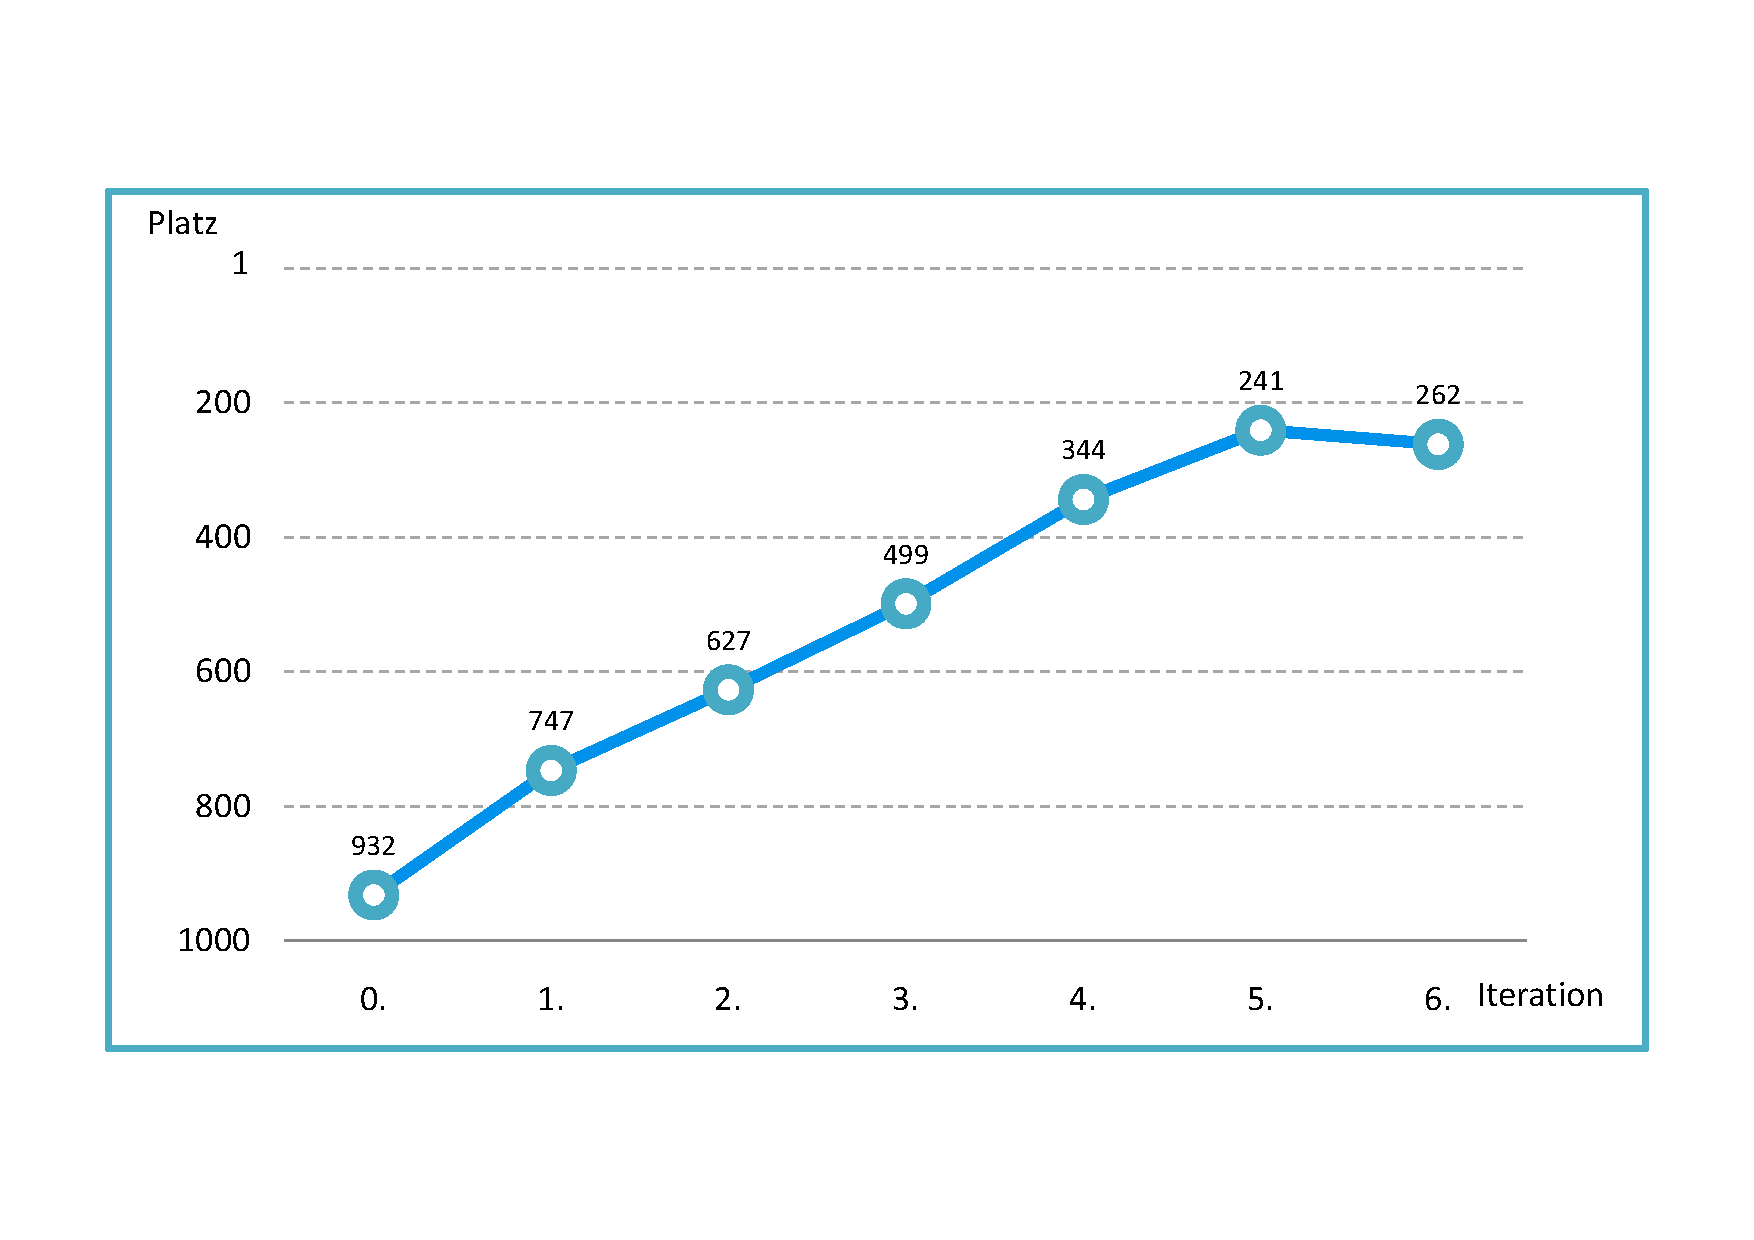
\includegraphics[width=0.85\linewidth]{Bilder/Trenddiagramm_Platzierungen}
\caption{Trenddiagramm unserer Kaggle-Platzierung}
\label{fig:Trenddiagramm_Platzierungen}
\end{figure}

Wie im Diagramm zu sehen, konnte mit jeder der 5 ersten Iterationen die Qualität der Vorhersage verbessert werden. In Iteration 4 konnten wir die Ergebnisse der Gruppe aus dem Vorjahr schlagen und haben letztendlich mit Iteration 5 unsere bisher beste Platzierung erreicht.

Die Auswahl eines Projektes auf der Plattform Kaggle.com, hatte für uns den besonderen Vorteil, dass wir unsere Ergebnisse direkt bewerten lassen konnten, auch wenn der Wettbewerb bereits beendet war. So konnte nach jeder Änderung geprüft werden, ob die Vorhersage verbessert wurde oder nicht. Zudem Bestand hier die Möglichkeit, sich mit Data-Mining Experten zu messen.

Generell gab die Veranstaltung einen guten Einstieg in die Verarbeitung großer Datenmengen und die dafür nötigen Werkzeuge. Es bleibt die Erkenntnis das es ein sehr umfassendes Gebiet ist, so dass für ein erfolgreiches Arbeiten in dem Bereich mehr als eine Veranstaltung nötig ist, um einen wirklichen Einstieg zu schaffen.